\documentclass[11pt]{article}
\usepackage[T1]{fontenc}
\usepackage[margin=1in]{geometry}
\usepackage{amsmath,amssymb}
\usepackage{graphicx}
\usepackage{booktabs}
\usepackage{xcolor}
\usepackage[colorlinks=true,linkcolor=blue!60!black,urlcolor=blue!60!black]{hyperref}
\newcommand{\code}[1]{\texttt{#1}}

\title{Self-Gravity with Mesh Refinement in the AthenaK Shearing Box\\
       \large Program Summary: Phases 0--3 --- Collapse, and the Stratified
       Gravito-Turbulent Box}
\author{\code{athenak-multigrid} tree, branch \code{multigrid}}
\date{August 25, 2026}

\begin{document}
\maketitle

\section*{Goal and route}
Target science: shearing-box simulations of gas + dust with self-gravity and
AMR zoom-in on gravitationally induced dust clumps (streaming-instability /
GI-arm interaction, cf.\ Baehr, Zhu \& Yang 2022), and the Gammie (2001)
gravitoturbulence program. Chosen route: a \textbf{multigrid Poisson solver
with shear-periodic boundary conditions on refined meshes}, with a
uniform-grid \textbf{FFT solver as the machine-precision oracle} throughout.
All work is validated against analytic solutions, the FFT oracle, and the
published Athena++ results the solver descends from (Tomida \& Stone 2023).
Full details: \code{multigrid\_selfgravity\_validation.pdf} (32 pp.),
reproduced end-to-end by \code{multigrid\_validation\_tests.ipynb} (44 code
cells); the FFT track has its own companion document.

\section*{Phase 0 --- shearing box + mesh refinement infrastructure (hydro)}
\begin{itemize}\itemsep2pt
  \item \textbf{Orbital-advection toggle}: a fully consistent non-FARGO mode
        (measured cost $5.7\times$: CFL against the full shear flow), enabling
        A/B tests and future patch refinement.
  \item \textbf{Refinement policies}: interior-$x_1$ / uniform-boundary-level
        rule (both shear faces share one level), and the \emph{annular} policy
        under FARGO --- refined regions span complete azimuthal rings, so the
        per-level $y$-shift only ever involves same-size neighbors.
  \item \textbf{AMR}: shear-boundary communication state rebuilt after every
        remesh; a graded-refinement cap keeps 2:1 balancing off the boundary
        columns; an upstream derefinement-ordering bug (partial ring splits)
        found and fixed.
  \item \textbf{Validation}: ring SMR bit-identical to reference runs; 20-orbit
        epicycle endurance --- amplitude drift $0.008\%$ (ring+FARGO) vs.\
        $0.064\%$ (uniform); AMR with a prescribed moving ring: 2296 blocks
        created / 2240 destroyed over 20 orbits, mass conserved exactly,
        matches the static ring an order of magnitude closer than either
        matches the uniform grid.
\end{itemize}

\section*{Phase 1 --- shear-periodic multigrid boundary conditions (uniform)}
Shear-periodicity enters as a boundary \emph{identification} only: a
$y$-remapped $x_1$ ghost fill (conservative PPMX remap) applied at every level
of the multigrid hierarchy through global boundary planes; the 7-point operator
is untouched. Key results: solves at shear-periodic instants are
\textbf{bit-identical} to plain-periodic solves; the analytic shearing-wave
potential is recovered \emph{below} the FFT solver's own error
($9.5\times10^{-8}$ vs.\ $1.6\times10^{-6}$ at $128^3$); the swing-amplification
history matches FFT to $2\times10^{-7}$; V-cycle contraction degrades only
$0.116 \to 0.157$ under a near-worst shear phase. Anchored to Tomida \& Stone
(2023): their \S4.1 convergence factor ($0.125$), second-order accuracy
(identical to FFT to all digits), and \S4.3 Jeans-wave results all reproduce.

\section*{Phase 2 --- multigrid gravity on refined shearing-box meshes}
\begin{center}
\small
\begin{tabular}{@{}lll@{}}
\toprule
phase & configuration & headline validation \\
\midrule
2a & static interior rings & guard-only change; ring solves bit-identical to \\
   & (boundary blocks at root) & periodic twins at $\mathrm{qomt}=0$; $L_2$ 2nd order; \\
   & & swing peak shifts \emph{toward} theory, gravity-off \\
   & & control dominates $\Rightarrow$ solver adds no error \\
2b & boundary annuli (refined & sheared octet ghost fill (host-side, rank- \\
   & blocks \emph{on} the shear faces) & replicated, no MPI seam); bit-identity at 1 and \\
   & & 2 levels; contraction unchanged ($0.18$--$0.20$) \\
2c & AMR & shear planes/offsets/octet flags rebuilt per \\
   & & remesh; moving-ring swing: several hundred \\
   & & remeshes, no solver warnings; $\mathrm{np}{=}2$ $\equiv$ serial \\
   & & to every printed digit \\
\bottomrule
\end{tabular}
\end{center}
The octet (refinement) machinery inherited with AthenaK \#776 was first
anchored on the isolated binary-potential test (T\&S \S4.2): region-wise
second order against the analytic two-sphere solution. Throughout Phase 2 the
refinement interface --- not the shear --- owns the error budget, and every
dynamic test carries a gravity-off control proving the gravity solver
contributes nothing beyond hydro truncation. One practical finding: refined
meshes should run FMG with a \emph{fixed} V-cycle count (T\&S practice); the
stagnation-exit stopping rule can hit its iteration cap mid-run on wound-up
shear modes.

\begin{figure}[htbp]
\centering
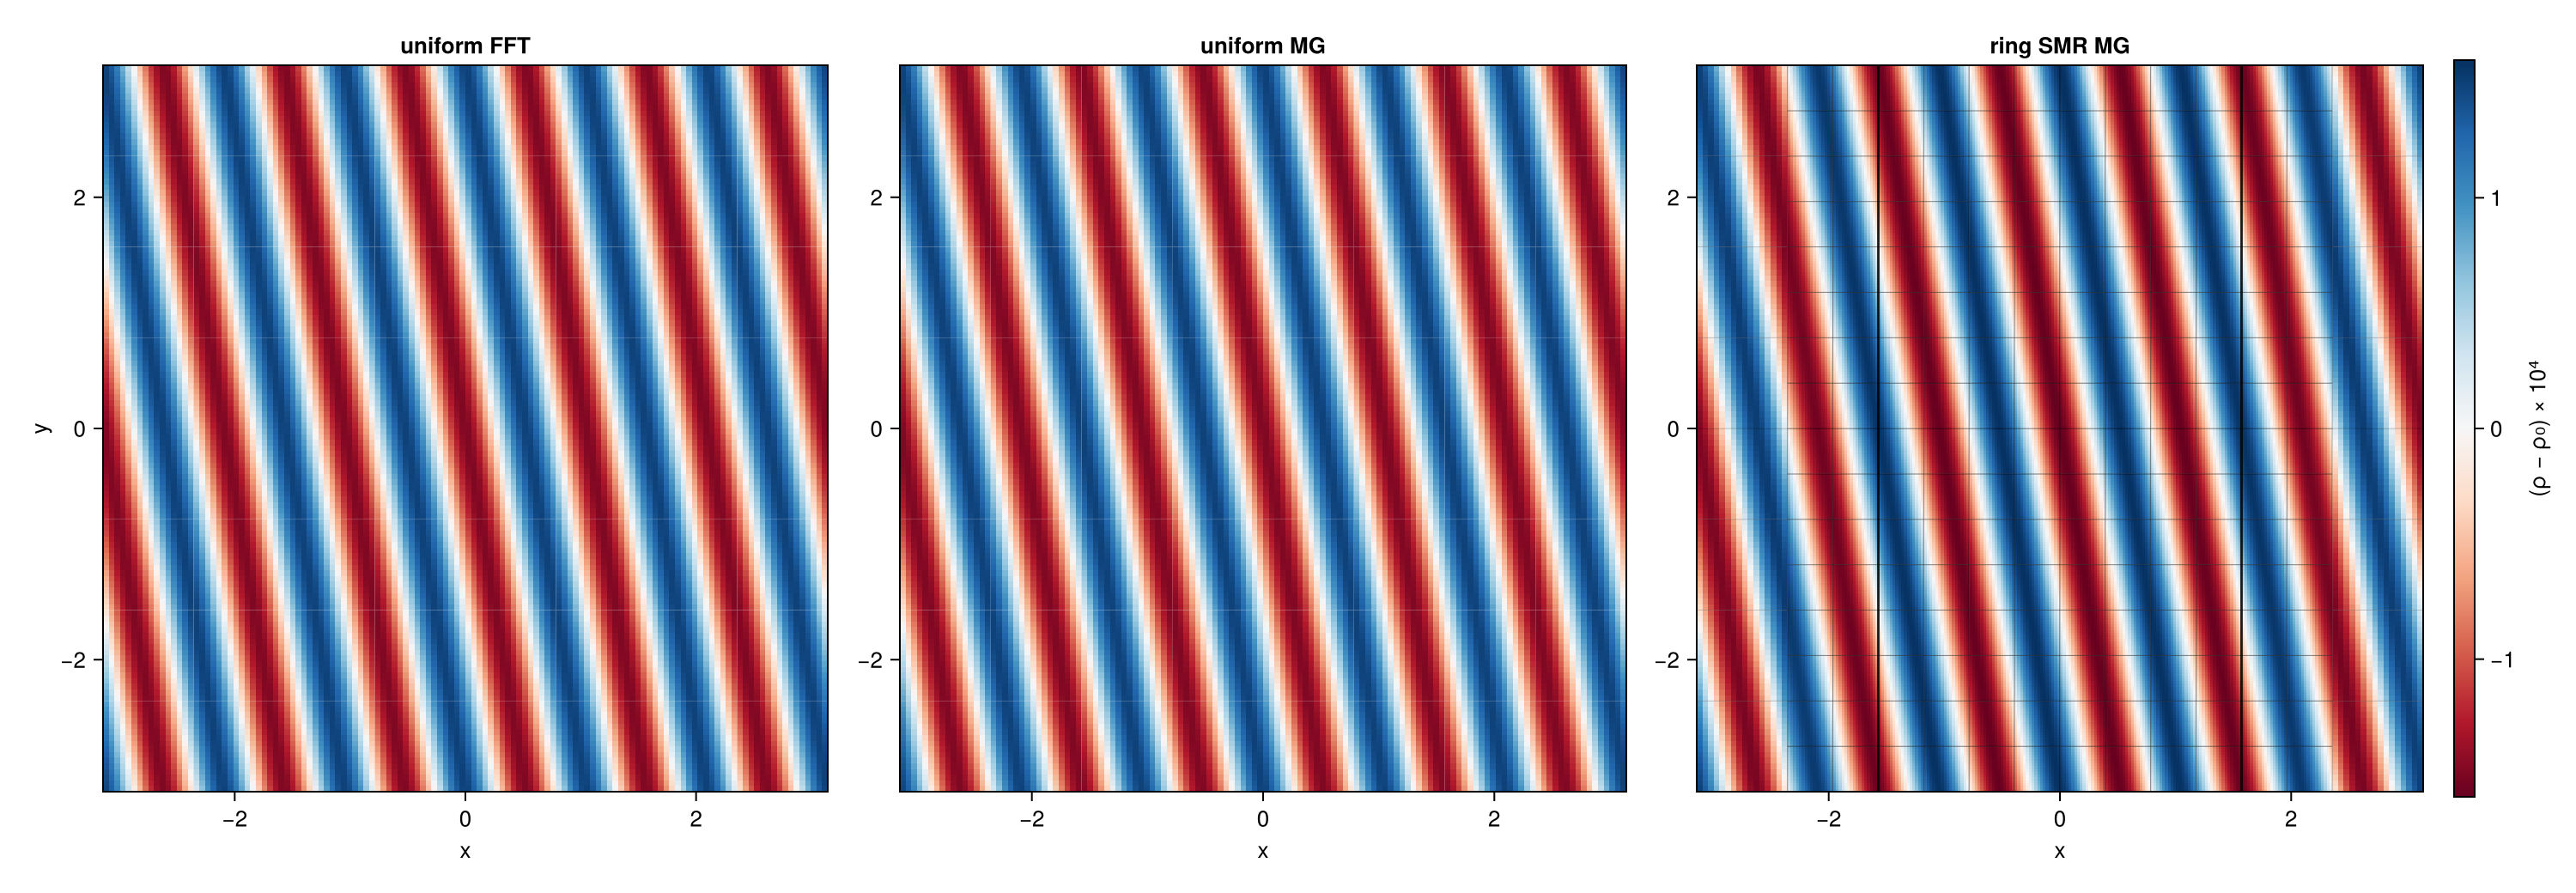
\includegraphics[width=\textwidth]{figures/mg2a_swing_dens.png}
\caption{The Phase-2a swing test: final density for uniform FFT, uniform
multigrid, and ring-SMR multigrid --- the two uniform panels agree at the
float32 quantization floor, and the wave crosses every refinement boundary
without artifact.}
\end{figure}

\section*{Into the unstable regime: first collapse (this week)}
With the machinery validated, the swing test was pushed past the box-scale
Jeans threshold ($4\pi G > \kappa^2 + k^2c_s^2 = 2$). An empirical ladder
established what clumping actually requires: transient waves \emph{bounce}
unless the compressed crest itself becomes Jeans-unstable during the unstable
window ($\lambda_J(\rho_{\rm crest})$ below the crest width). At
$4\pi G = 6$, amp $= 0.2$ the crest fragments at $t \approx 4.5$ and collapses
into a \textbf{bound clump at $\rho = 203\rho_0$} --- beyond the uniform-grid
Truelove ceiling ($171\rho_0$), motivating the AMR zoom, which follows the
crest and clump with density-triggered rings (the annular policy answers
``how do you zoom under FARGO'': rings, completed automatically by the
flag-sync, not local patches). The multigrid solver ran the entire collapse
--- a 200:1 density contrast on a shear-periodic adaptive mesh --- with zero
convergence failures.

The program is now \textbf{deployed on NAS HECC}: a $256^2$ discriminator run
at 64 ranks confirmed the two-site fragmentation as physical (the $128^2$
single clump was an under-resolution artifact), and its $t{=}14$ extension
followed the winner-takes-all endpoint --- runaway to $2.6\times10^5\rho_0$
with the companion consumed --- with the solver machine-clean through the
quarter-million contrast. The deployment also exposed (deterministically, at
the same timestep in two attempts) a latent \textbf{upstream bug} in the
shearing-box $x_1$ exchange: sender and receiver computed the integer shear
shift from their own MeshBlocks' stored cell sizes, whose last-ulp roundoff
can disagree near integer crossings, desynchronizing MPI message sizes. All
seven shift computations now derive from bitwise-identical global mesh
quantities; the fix is validated from serial (bit-identical to prior
references) to 64 ranks.

Finally, an \textbf{FFT-solver cross-check} closed the last audit channel:
a serial FFT twin of the $256^2$ collapse matches the multigrid run to
$5\times10^{-8}$ through the linear phase and reproduces the \emph{same two
fragments within a third of a cell} after five nonlinear dynamical times;
extended to $t{=}14$, both solvers reach the same fate on the same clock
($\rho{=}100$ crossings within $0.05$), diverging only \emph{beyond} the
Truelove ceiling (FFT saturates near it; multigrid runs away unresolved) ---
a solver-based demonstration that past-ceiling densities are resolution
artifacts. The $y$-boundary fragmentation has now survived four independent
audits: resolution, mesh topology, rank count, and solver identity.

\begin{figure}[htbp]
\centering
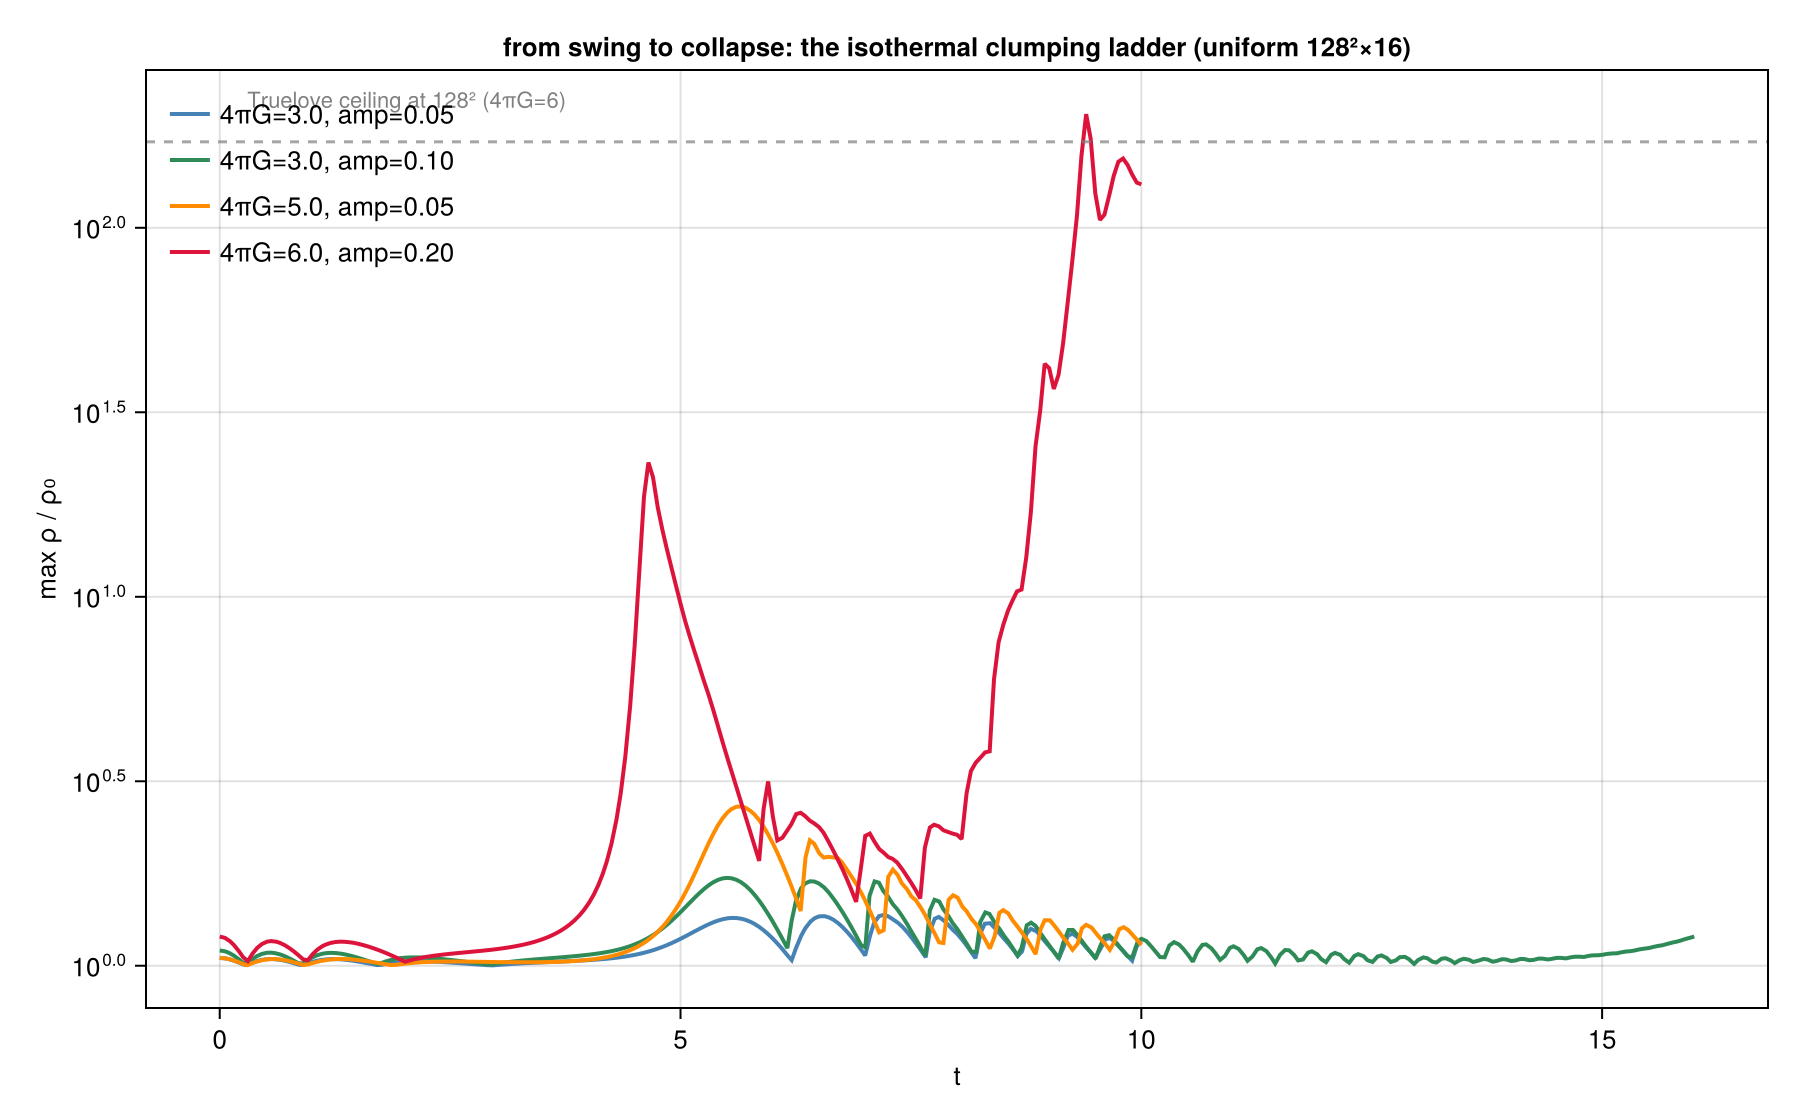
\includegraphics[width=0.72\textwidth]{figures/clump_ladder.png}
\caption{The nonlinear ladder: maximum density vs.\ time for the four
uniform-grid runs, with the Truelove ceiling marked.}
\end{figure}

\begin{figure}[htbp]
\centering
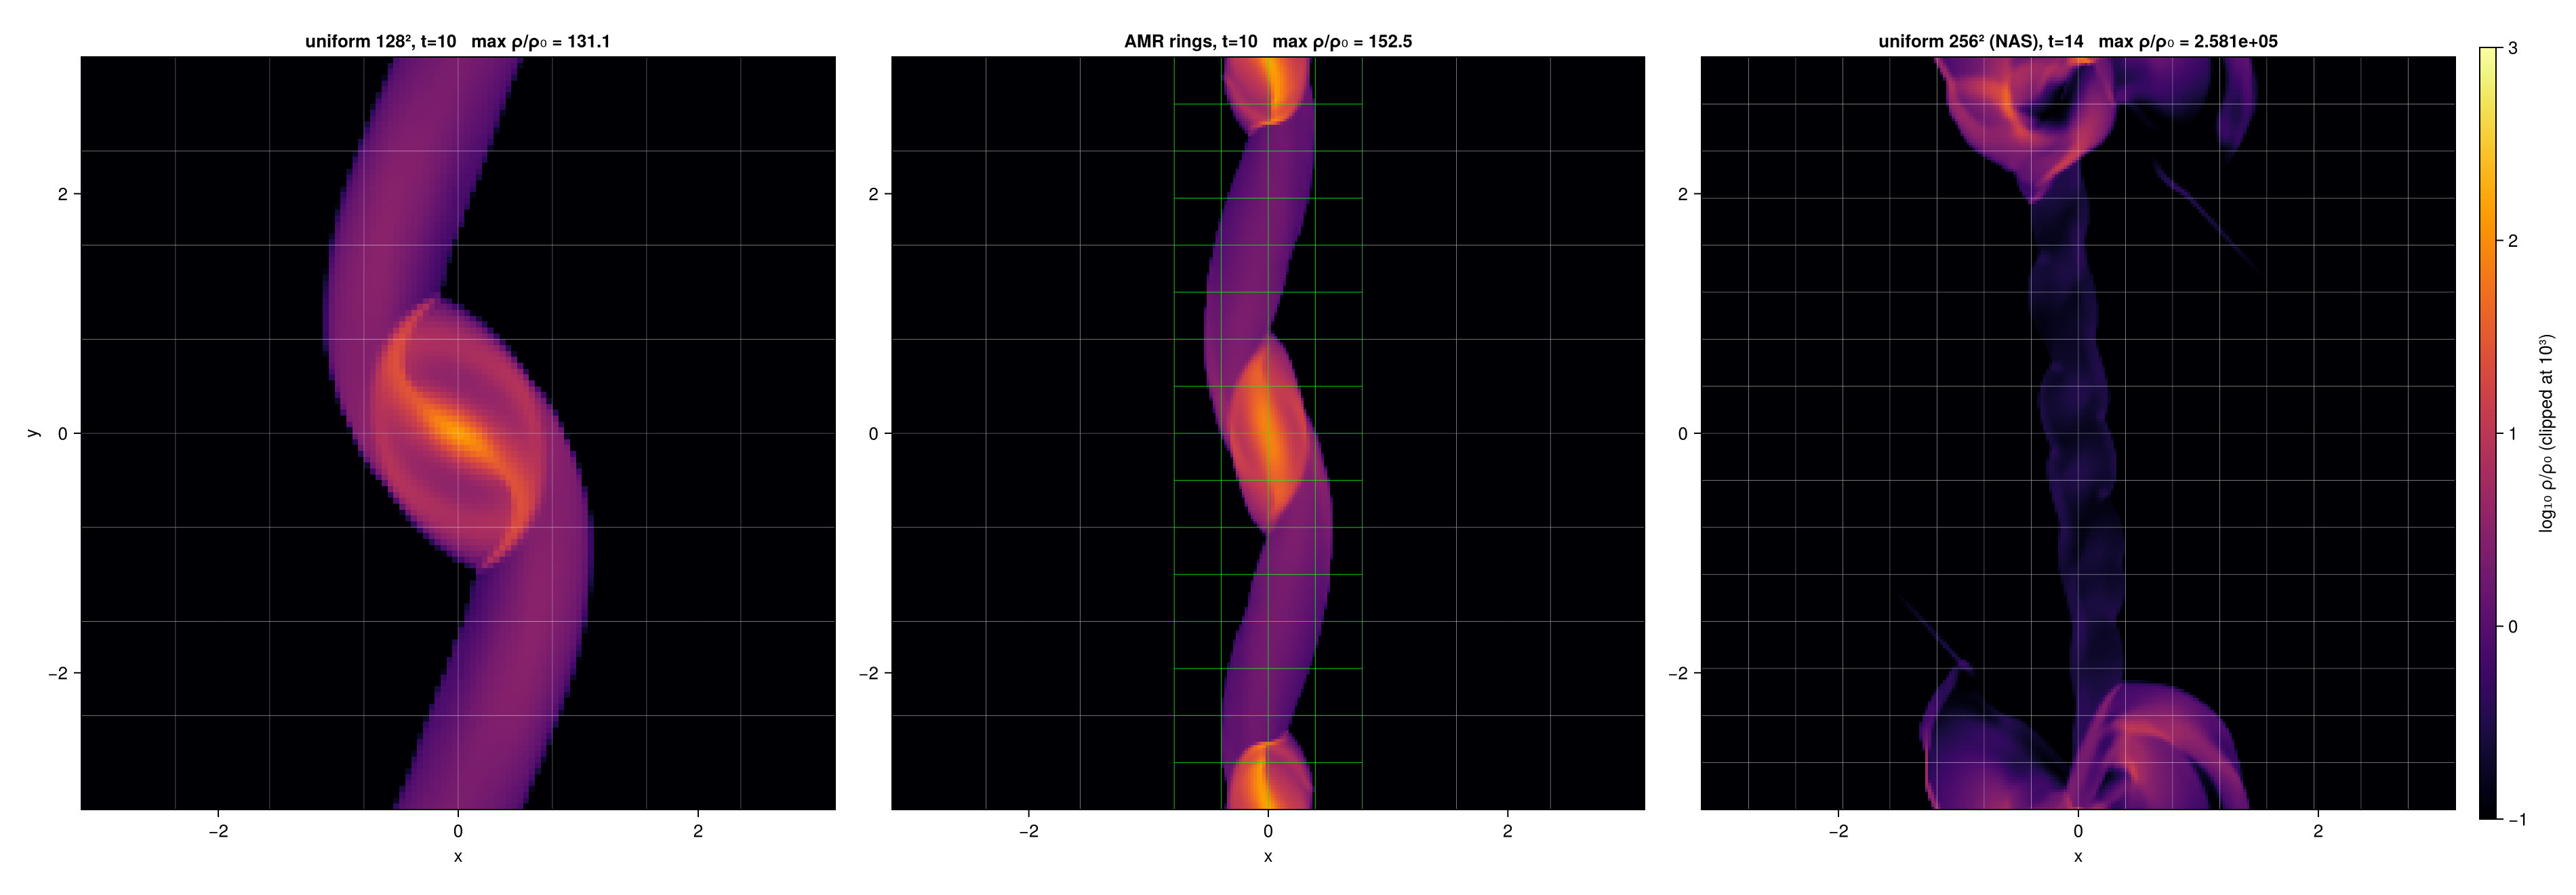
\includegraphics[width=\textwidth]{figures/clump_final3.png}
\caption{Final states of the collapse runs ($\log_{10}\rho$, MeshBlocks
drawn, green = level 1): uniform $128^2$ (fragments merged by
under-resolution), the AMR run resolving both clumps, and the $256^2$ NAS
run at $t=14$ in the winner-takes-all runaway.}
\end{figure}

\begin{figure}[htbp]
\centering
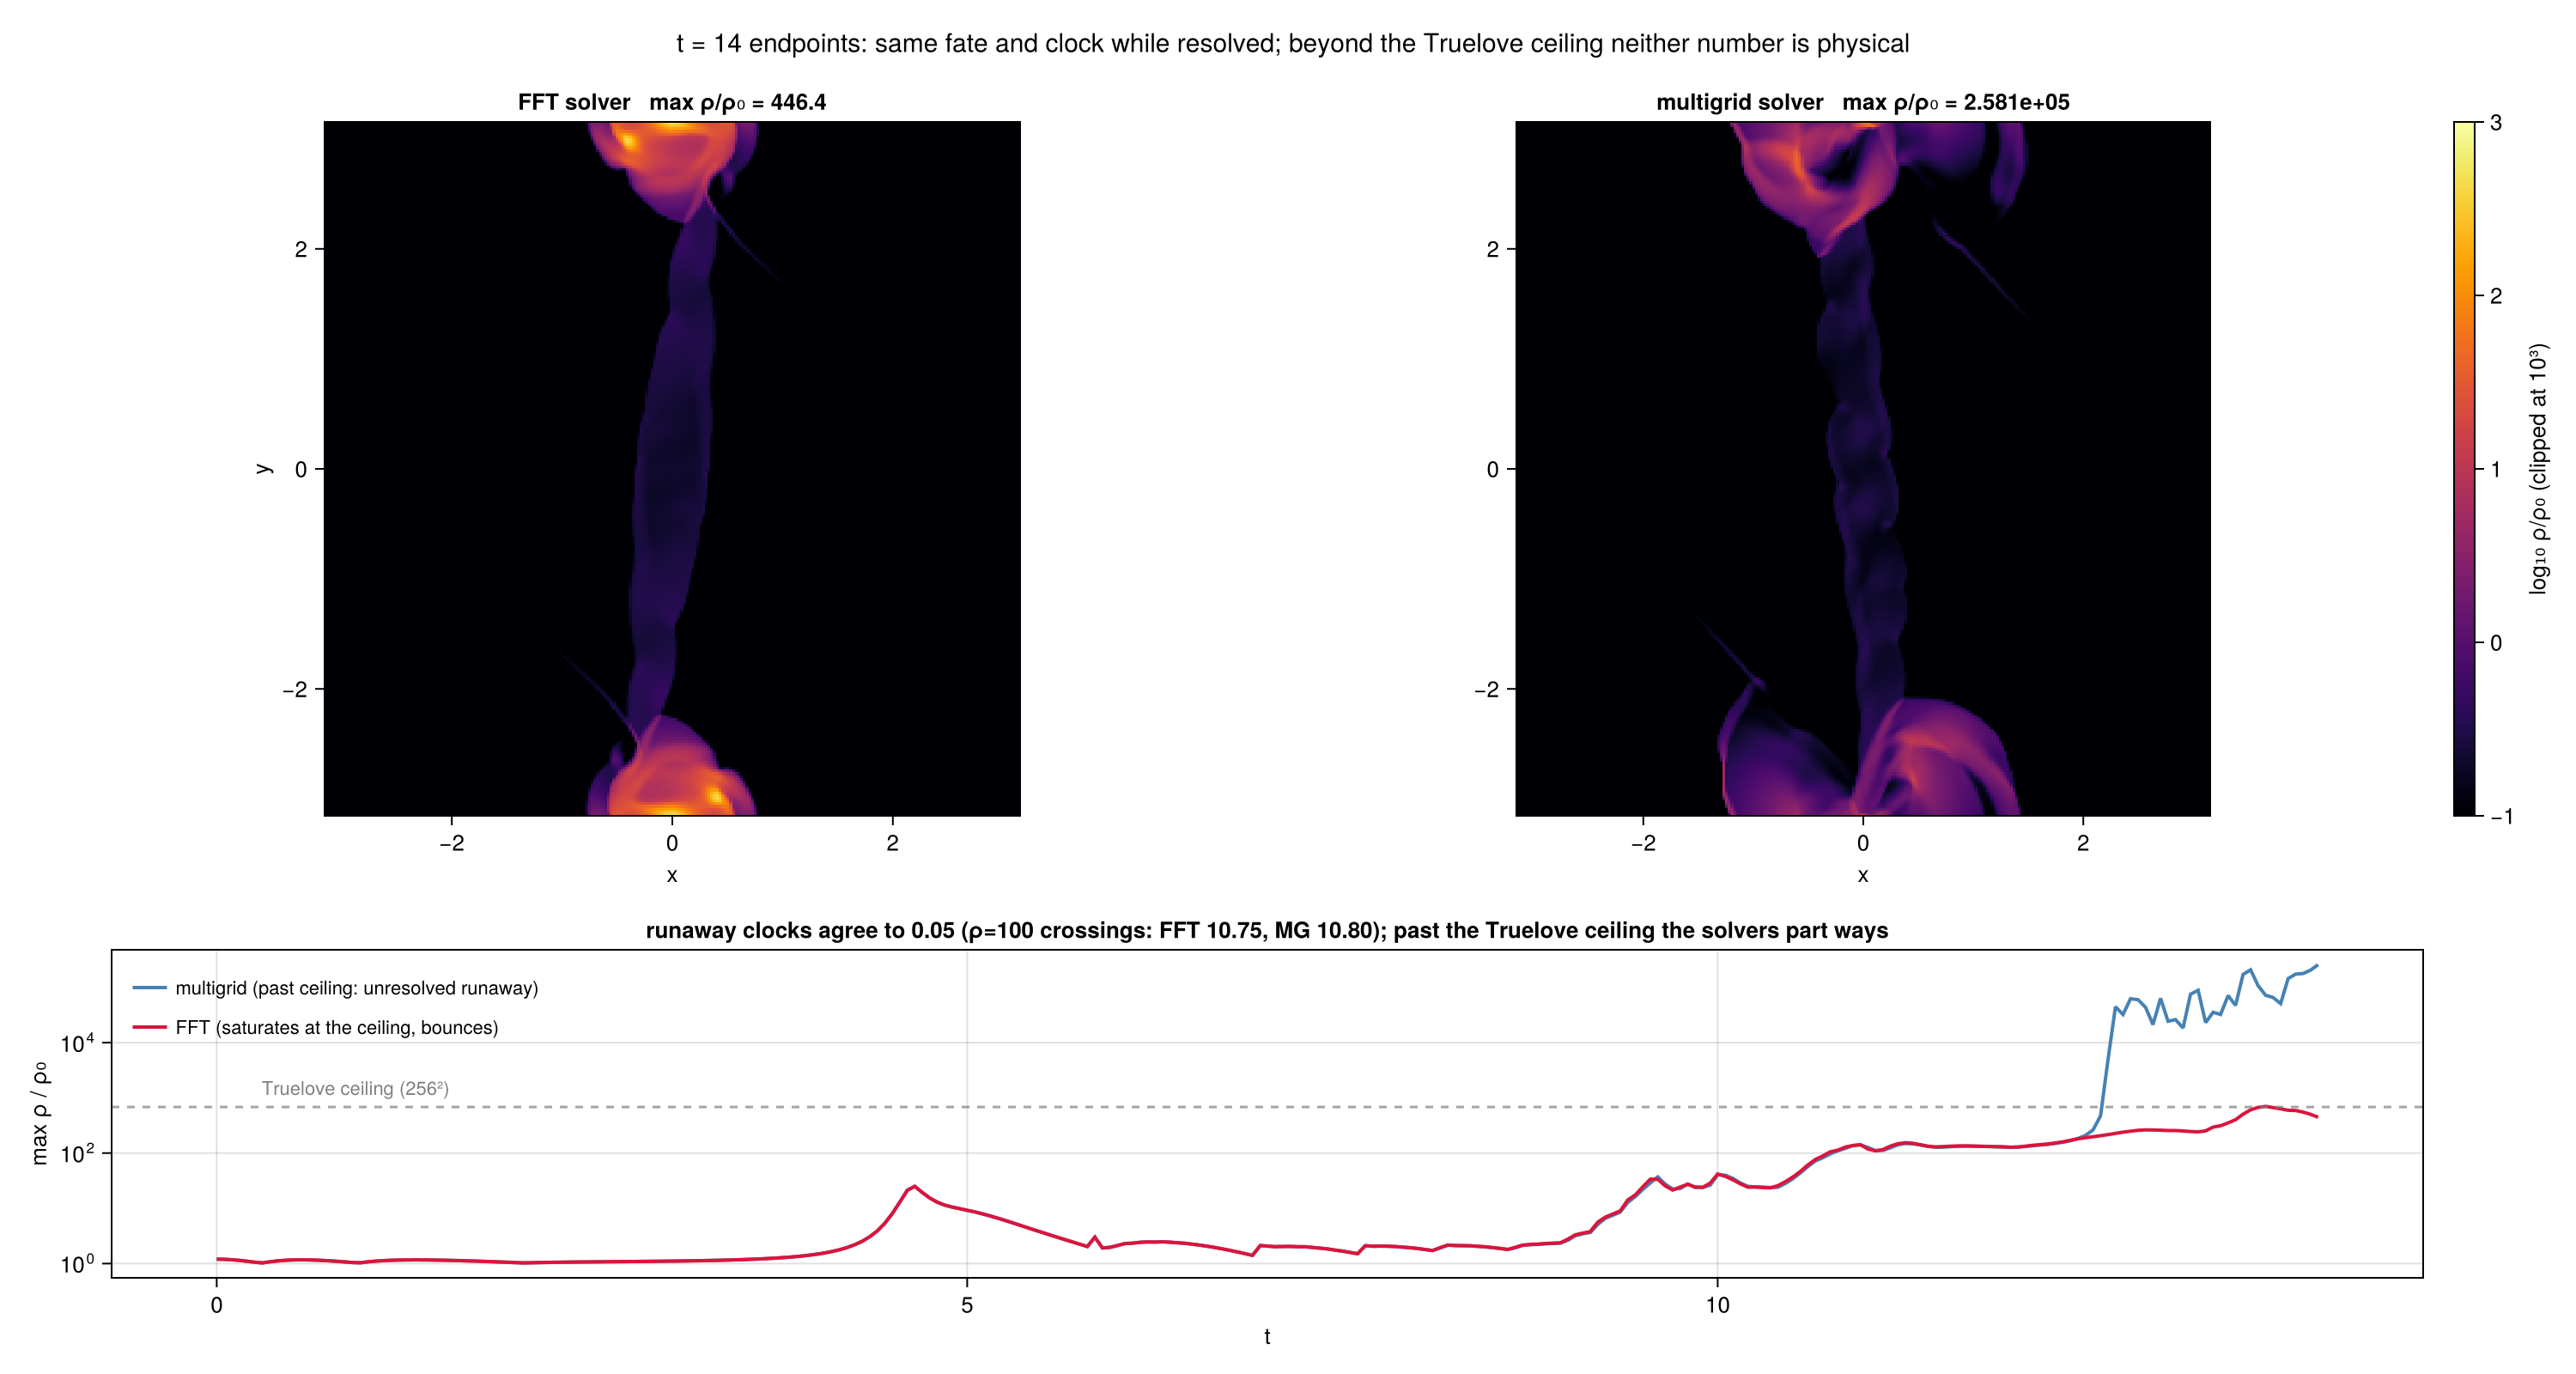
\includegraphics[width=0.9\textwidth]{figures/fft_vs_mg_endpoint.png}
\caption{The solver cross-check at $t=14$ (column-maximum density
projections): FFT and multigrid agree on fate and clock while the collapse
is resolved, and part ways only beyond the Truelove ceiling (dashed) ---
neither number is physical there.}
\end{figure}

\section*{Phase 3 --- the stratified box: slab-open gravity, cooling, and
gravito-turbulence (this week)}
The third dimension of the physical problem. Three deliverables:

\textbf{(i) Open (vacuum) vertical boundaries for the multigrid solver}
(\code{mg\_bc = slab}): each solve builds exact Dirichlet face planes from the
\emph{discrete} infinite-vacuum Green's function of the 7-point stencil
($\mu$-decay per horizontal mode at the shear-shifted $k_x'$; the discrete slab
potential for the now-physical mass sector), applied at every multigrid level.
The converged interior equals the infinite-domain discrete solution
\emph{exactly}: a new closed-form ``sheet'' arbiter validates this absolutely
(no mean subtraction) at $1.2\times10^{-12}$, against the independent FFT-KO09
method at $3\times10^{-13}$, bit-identically across MPI ranks, and at
$8\times10^{-5}$ through five dynamical times of \emph{nonlinear evolution}.
Shear, SMR, and dynamic AMR all compose with it; the only refinement cost is a
constant \emph{force-free} $O(h^2)$ offset in enclosed refined regions --- the
dipole signature of the conservative level interface, invisible to every
periodic-box test that came before.

\textbf{(ii) Stratified-box physics}: the vertical tidal force's missing energy
work term (a latent upstream gap, invisible to isothermal runs), SC14's two
cooling laws with timestep guards, and a boundary lesson --- plain
\code{outflow} $z$-boundaries feed a gravity-driven \emph{inflow runaway}
(halo mass up $100\times$, disk destroyed by $t\sim8\,\Omega^{-1}$); the
\code{diode} boundary makes the SC14 initial state hold hydrostatically to
$2\%$ of $c_s$. AMR refinement is automatically vetoed on the $x_3$ faces, and
a clump-triggered AMR run tracked collapse clumps through refine/derefine
cycles with the slab planes rebuilt at every remesh.

\textbf{(iii) The Shi \& Chiang (2014) reproduction}: a \code{gravito\_turb}
pgen integrating their self-gravitating vertical equilibrium (their published
constants reproduce the $Q_0{=}1$, $H{=}1$ calibration to $5\times10^{-4}$ ---
an independent audit of the paper), with their $Q$, $\alpha$ (eq.~19),
$\alpha'$ (eq.~20) diagnostics as history outputs. The half-width production
run ($[-16,16]^2{\times}[-6,6]H$ at their resolution, $\beta = 10$, 4 MPI
ranks, $6.8$\,h on a laptop) reproduces their Figure~2 end to end
(Fig.~\ref{fig:sc14}): cooling collapse, vertical rebound, then
$250\,\Omega^{-1}$ of self-regulated gravito-turbulence with, over their
averaging window, $\langle c_s\rangle_\rho = 2.187$ (theirs: $2.18$), rms
$\delta v = 1.68\,H\Omega$ ($1.79$), $M/M_0 = 0.92$ ($\sim0.9$), and
$\alpha_{\rm grav} = 0.034$ ($0.039$). The residual gaps ($Q = 1.11$ vs
$1.33$; a burst-inflated Reynolds channel) all carry the signature of a single
box-scale swing mode recharging quasi-periodically --- the half-width-box
effect --- which the \textbf{full-width $64H$ run now queued on NAS} will
resolve; the $\beta$-scan (their Table 1, via their ``morphing'' restart
chain) is packaged alongside it (\code{scripts/cluster/}).

\begin{figure}[htbp]
\centering
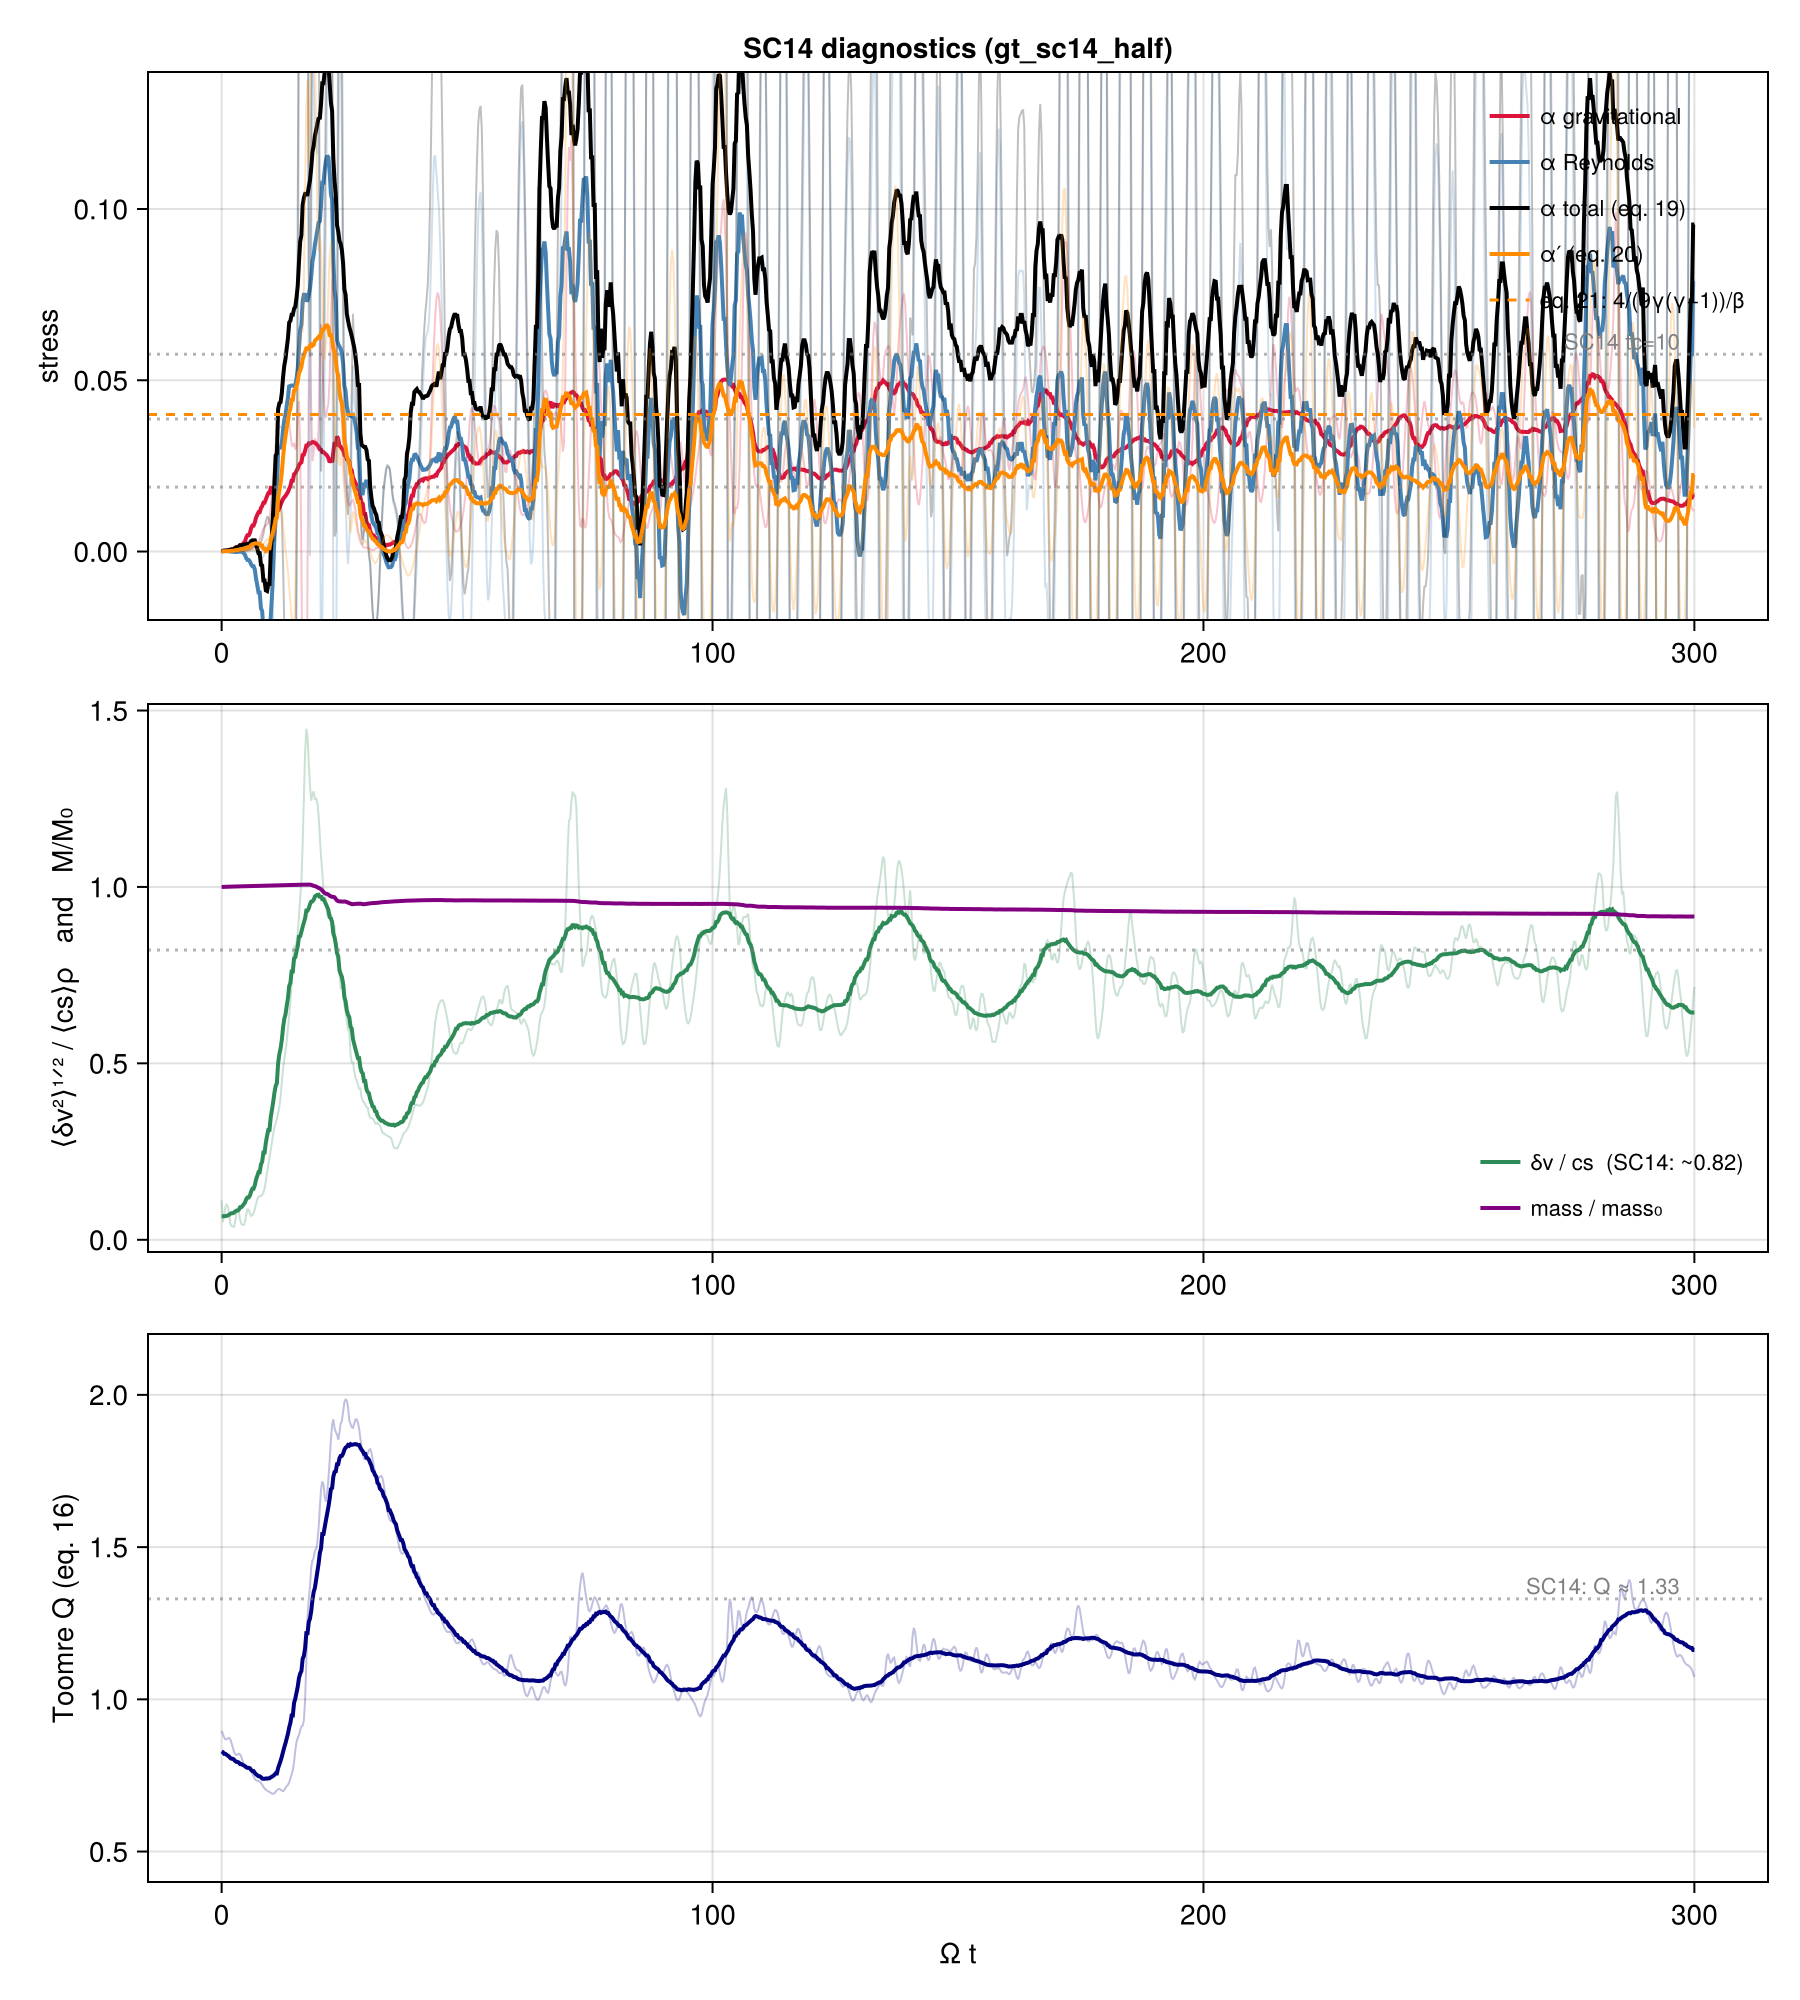
\includegraphics[width=0.9\textwidth]{figures/sc14_half_hist.png}
\caption{The SC14 $\beta = 10$ half-box run in their Figure-2 form (thick:
$12\,\Omega^{-1}$ boxcar; dotted: SC14's tc=10 values; dashed: their eq.-21
energy-balance line): stresses, $\delta v/c_s$ and mass, Toomre $Q$.}
\label{fig:sc14}
\end{figure}

\begin{figure}[htbp]
\centering
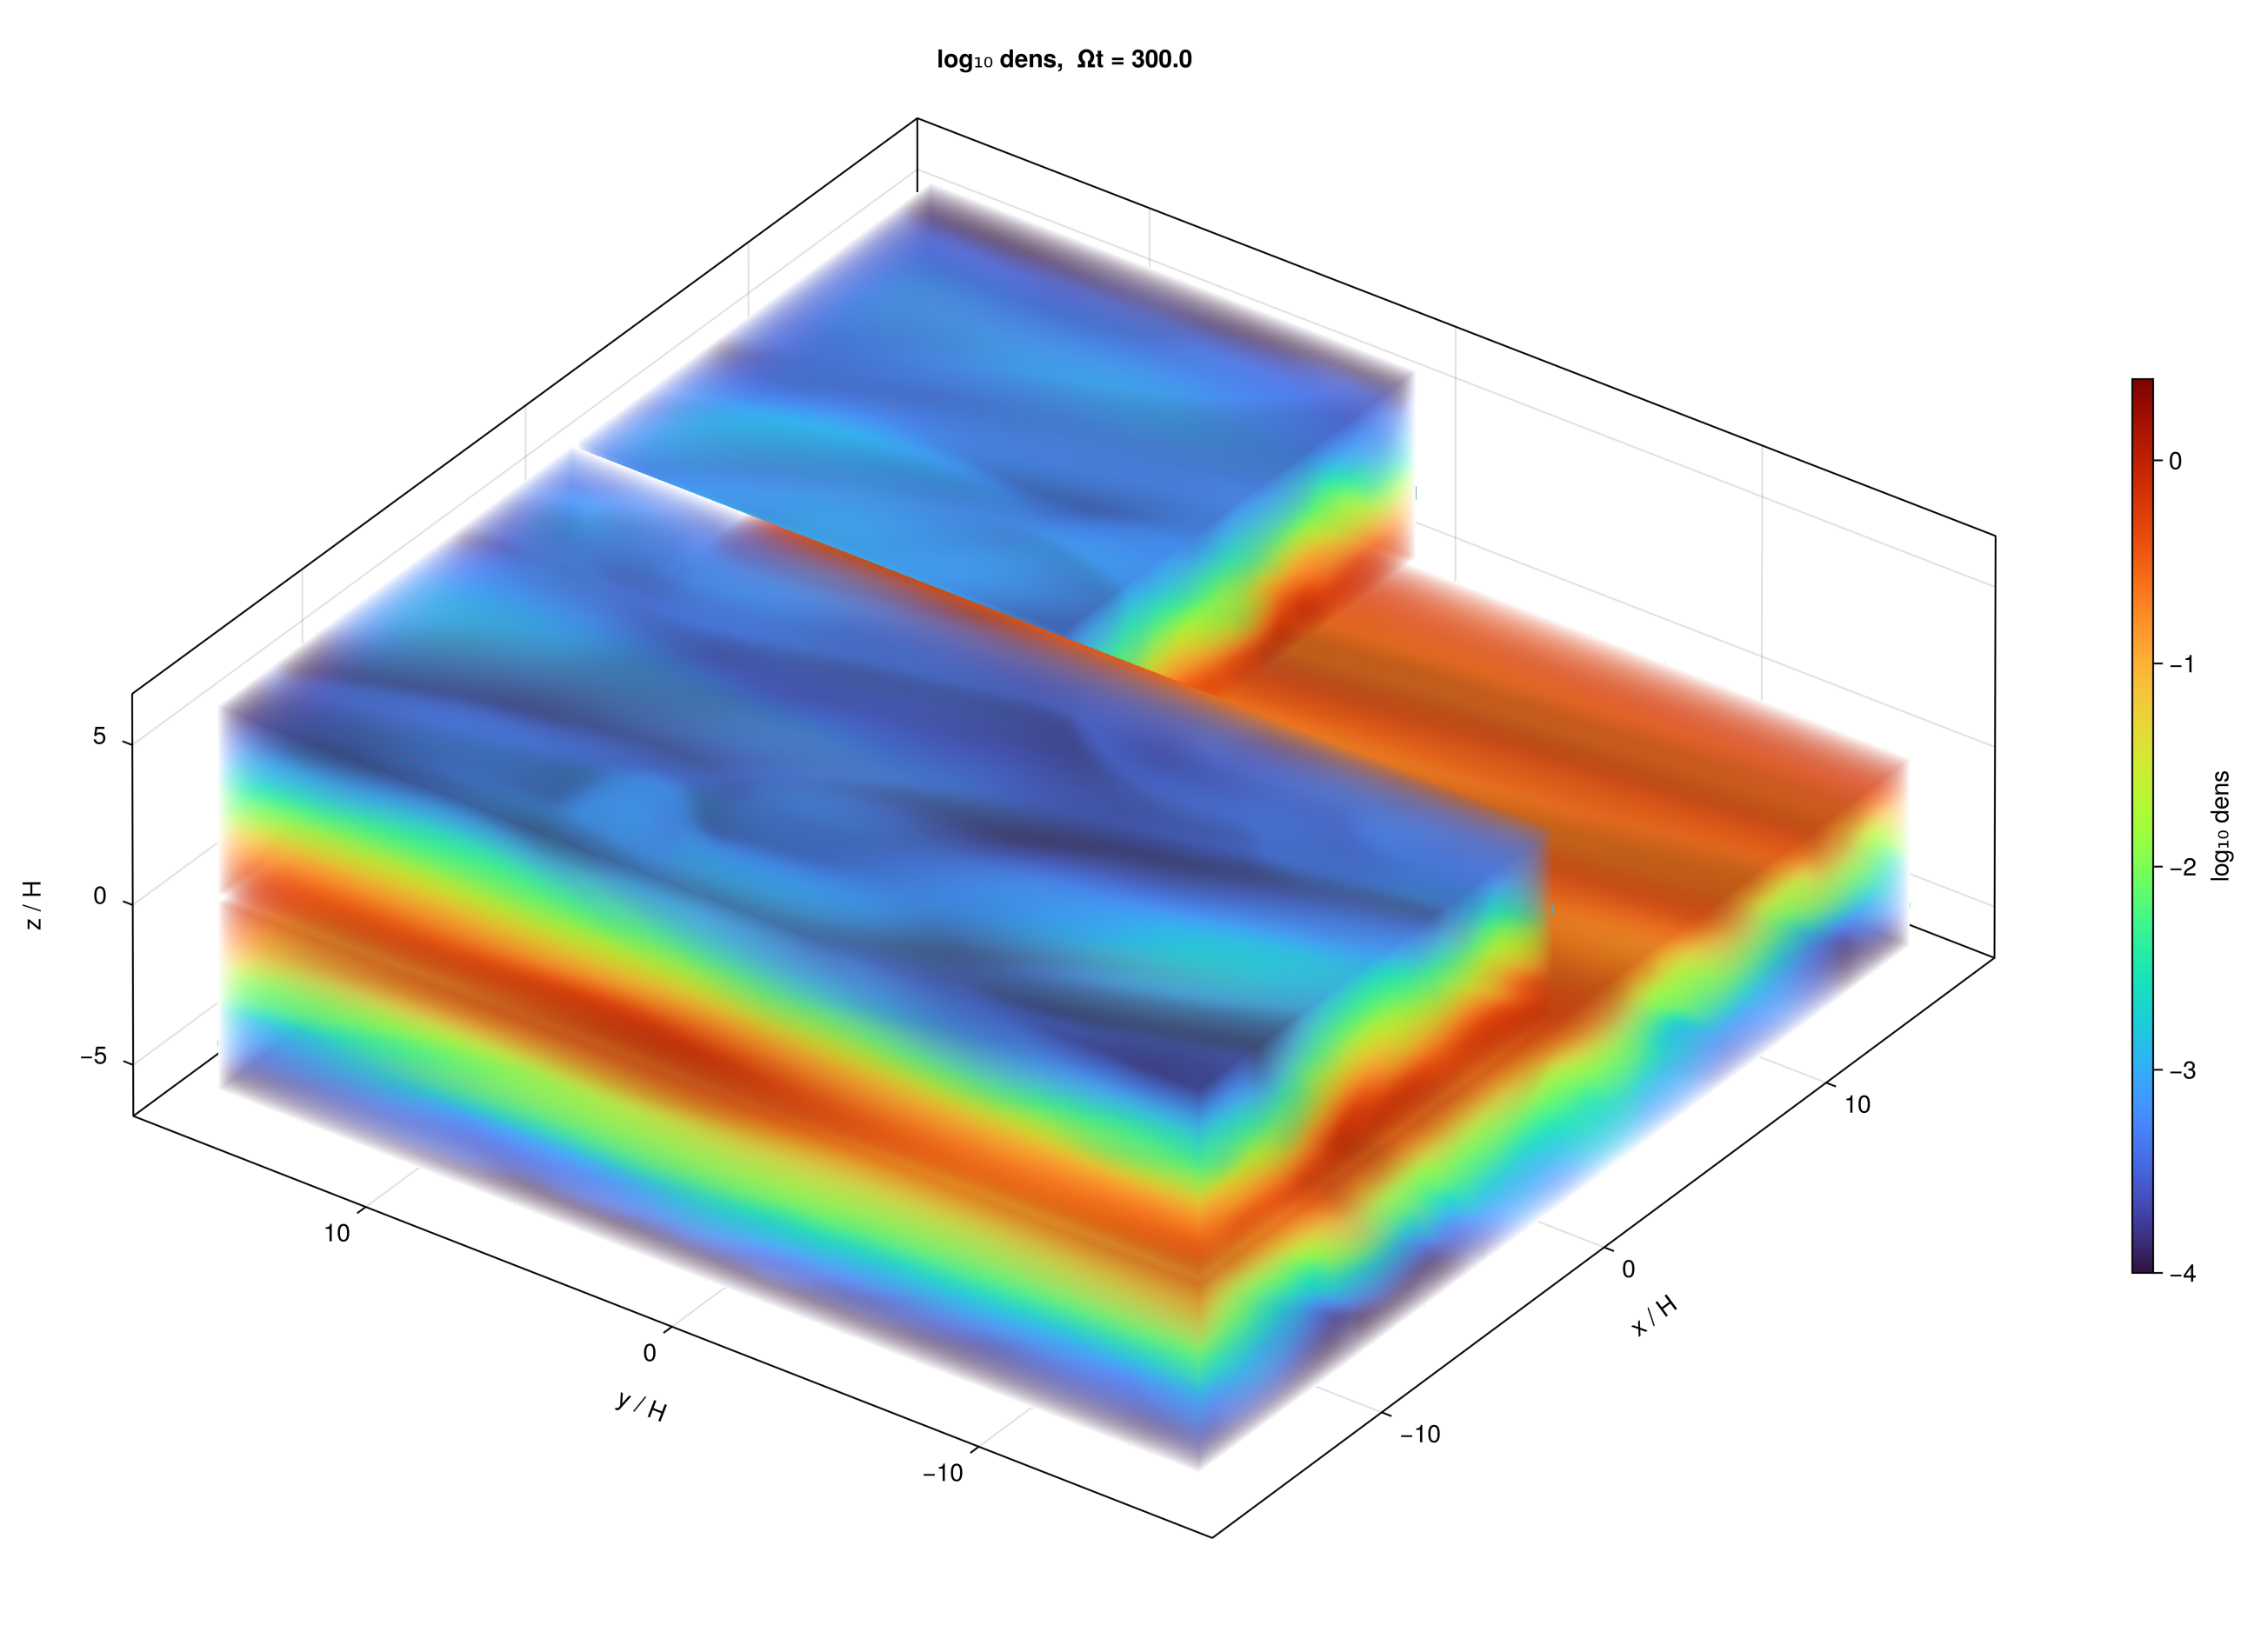
\includegraphics[width=0.85\textwidth]{figures/sc14_half_vol_cut.png}
\caption{$\log_{10}\rho$ at $\Omega t = 300$, cutaway volume rendering in the
style of SC14's Fig.~2: gravito-turbulent midplane wakes under the halo they
force --- the configuration (stratified, open-$z$, refinable) that no FFT
solver can host.}
\end{figure}

\section*{Status and next steps}
\textbf{Delivered}: FFT solver (validated, incl.\ open-$z$, and a full
nonlinear cross-check twin); shearing-box refinement infrastructure incl.\
AMR; multigrid gravity on uniform, SMR-ring, boundary-annuli, and adaptive
meshes, serial and MPI, now with slab-open vertical boundaries for stratified
disks; cooling; the SC14 configuration, analysis tooling, and cluster kit;
$\sim$40 pages of validation documentation, the reproducing notebook, and
versioned test inputs for every configuration.
\textbf{Next}: (i) the full-size SC14 runs on NAS ($\beta$-scan, resolution
doubling, and AMR zoom-in on gravito-turbulent clumps --- the configuration no
FFT code can run); (ii) dust coupling (athenak-dust PM particles + IMEX drag)
toward the SI+GI clumping science (Phases 4--5); (iii) deferred
infrastructure: host-root shear fill, MHD face-centered remap with refinement,
and (if deep zooms demand it) per-ring bookkeeping for patch refinement under
FARGO.

\end{document}
